\section{Related work}\label{sec:related-work}
There are many software and technologies that bring music into virtual reality or augmented reality applications,
from systems for playing virtual or semi-virtual instruments,
to virtual tutors evaluating the musical performance of a beginner musician.

\subsection{Virtual and semi-virtual instruments}\label{subsec:virtual-and-semi-virtual-instruments}
One of the most important features of VR and AR is to make the user interface with something that does not exist,
but at the same time is visible in a virtual or semi-virtual environment, with even the possibility of giving feedback
visual or tactile feedback in response to an action.

In~\cite{cyber-glove} Cyber Composer is proposed, an interactive cyber instrument to enable both musicians and music laypersons
to dynamically control the tonality and the melody of the music that they compose through hand motion and gestures.
This system is empowered by the embedding of music theories to ensure the music
generated makes musical sense in the perspective of musicians.

Two sensors are used to track hand movements: a pair of CyberGlove and a Polhemus FASTRAK 3D Position Tracker.
The CyberGlove provides high-performance hand measurements and real-time motion capture
thanks to bend and flexion sensors on fingers, palm, and wrist.
A Polhemus sensor is attached to each glove, to provide 3D positioning and orientation information.

The software consists of four components:
music interface, CyberGlove interface, background music generation module and melody generation module,
all linked together by the main program, which provides a user-friendly graphical user interface.

The system implements seven musical expressions, mapping each one to a different kind of motion of gesture with one or two hands.
The musical expressions are rhythm, pitch, pitch-shifting, dynamics, volume, dual instrument mode, and cadence.
The gestures used to control the generated melody include, among others, flexion of the right wrist,
height of the right hand relative to the ground and lifting of the same hand,
position of the left hand relative to the right hand, and bending the fingers of the left hand.

\begin{figure}[ht]
	\centering
	\begin{subfigure}{0.32\textwidth}
		\centering
		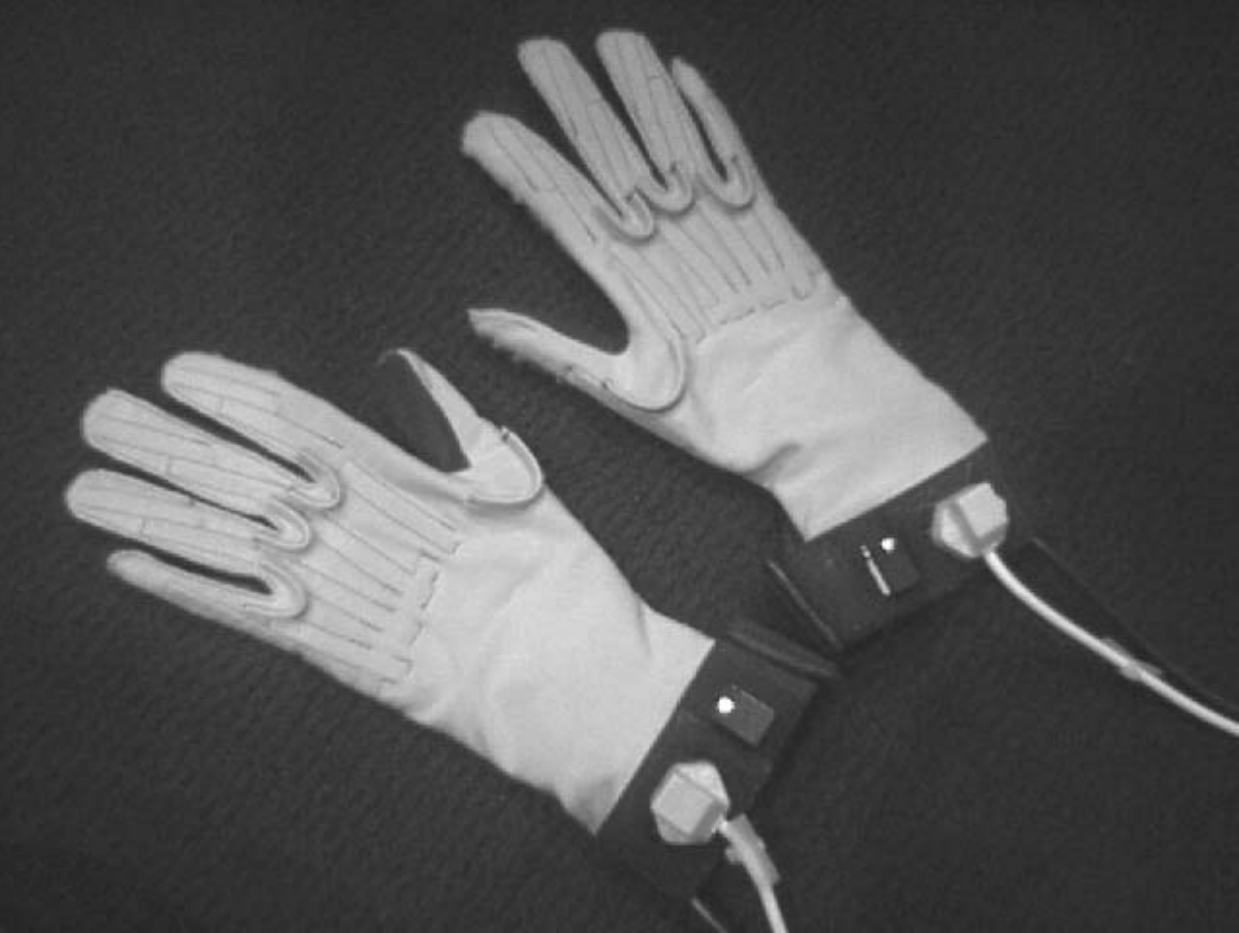
\includegraphics[width=\textwidth]{images/related-work/cyber-gloves}
	\end{subfigure}
	\hfill
	\begin{subfigure}{0.32\textwidth}
		\centering
		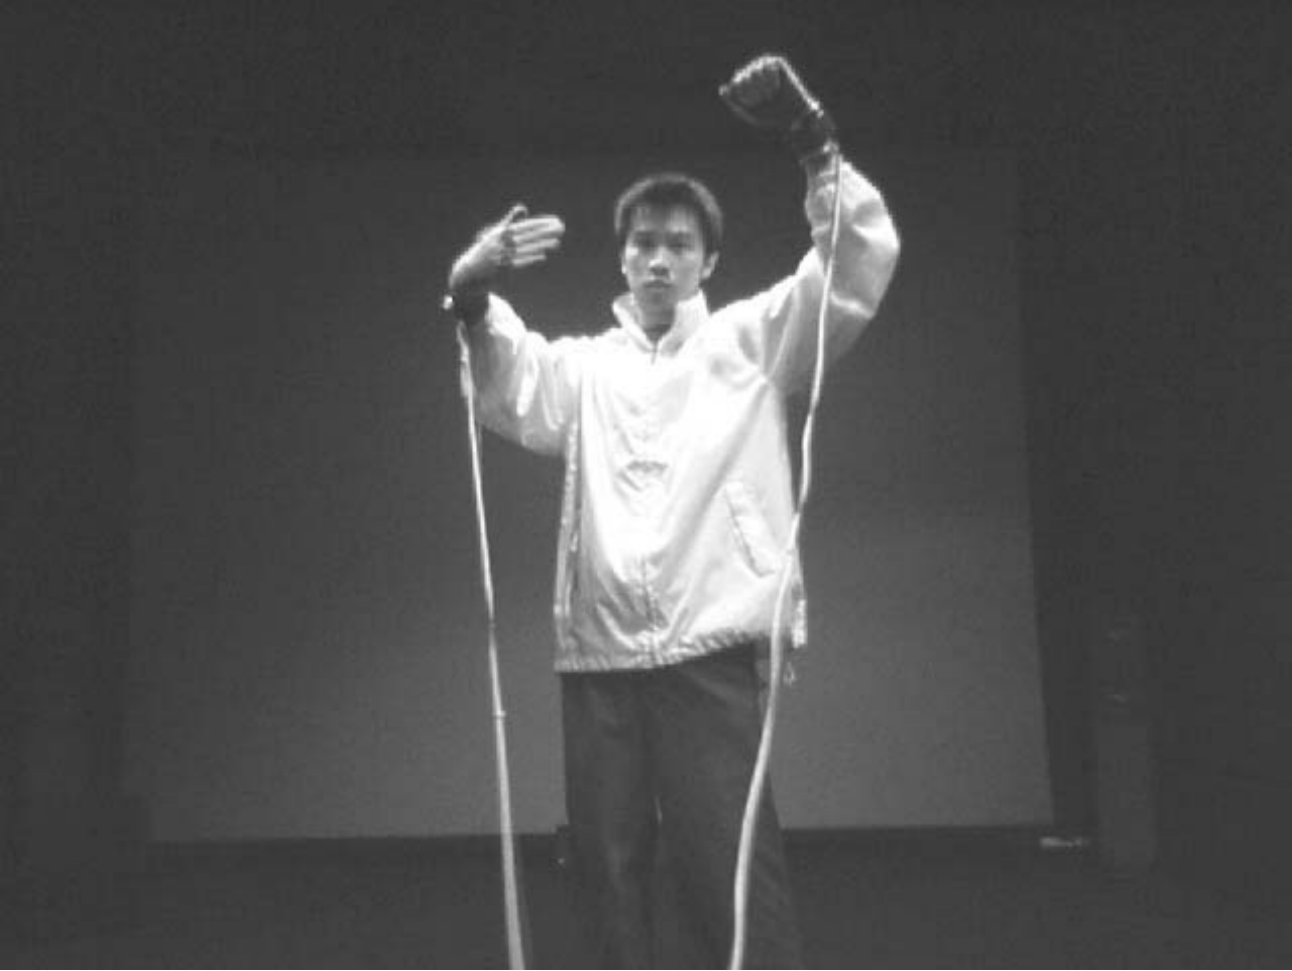
\includegraphics[width=\textwidth]{images/related-work/cyber-gloves-example}
	\end{subfigure}
	\hfill
	\begin{subfigure}{0.32\textwidth}
		\centering
		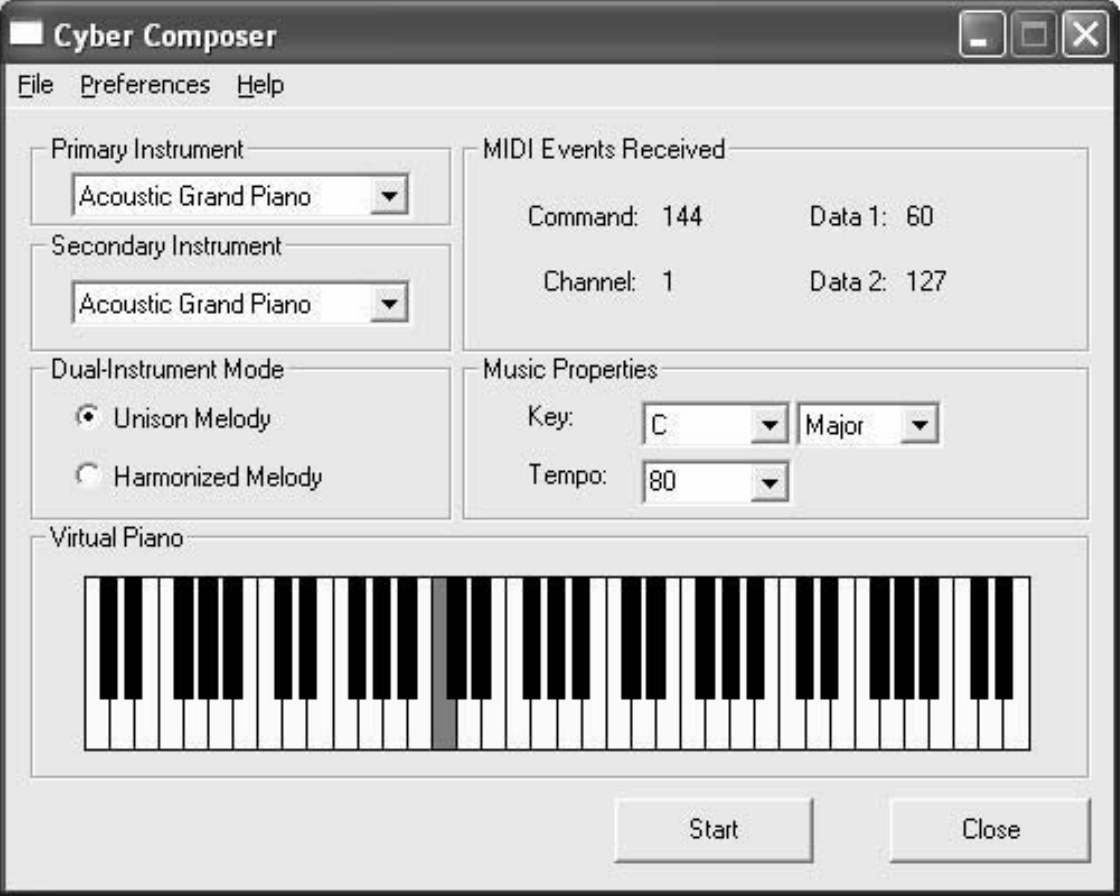
\includegraphics[width=\textwidth]{images/related-work/cyber-glove-gui}
	\end{subfigure}
	\caption{CyberGloves used in Cyber Composer~\protect\cite{cyber-glove} and its graphical user interface}
	\label{fig:cyber-glove}
\end{figure}

In~\cite{semi-virtual-instruments} two semi-virtual instruments based on physical interfaces are implemented:
a flute and a drum.

A semi-virtual flute is created using a real plastic tube with three buttons and a small fan inside,
which is activated by the user's breath.
The rotation of the fan is transmitted to the computer, which processes it together with the data on the buttons pressed,
producing the corresponding sound.
A drum, on the other hand, is created using only a stick with a red object attached to the tip.
The red tip is tracked by the webcam, which calculates its movement by keeping track of its position and speed.

Both the flute and the drum can be visualized live on the computer screen, accompanied by visual effects
which inform the user of the type of sound produced.

\begin{figure}[ht]
	\centering
	\begin{subfigure}{0.32\textwidth}
		\centering
		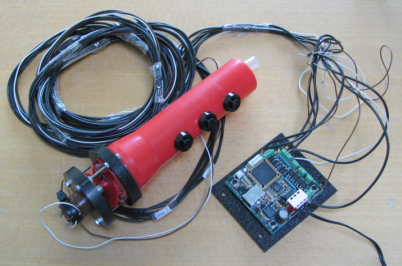
\includegraphics[width=\textwidth]{images/related-work/semi-virtual-flute}
	\end{subfigure}
	\hfill
	\begin{subfigure}{0.32\textwidth}
		\centering
		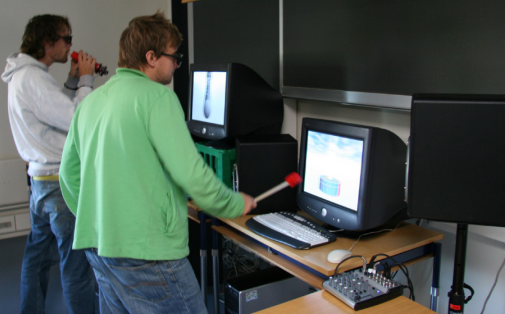
\includegraphics[width=\textwidth]{images/related-work/semi-virtual-drum}
	\end{subfigure}
	\hfill
	\begin{subfigure}{0.32\textwidth}
		\centering
		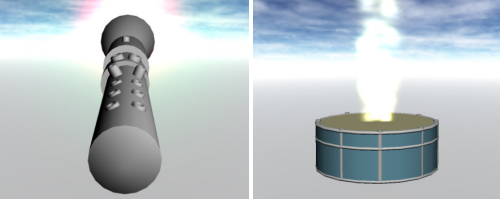
\includegraphics[width=\textwidth]{images/related-work/semi-virtual-visualization}
	\end{subfigure}
	\caption{Semi-virtual flute, semi-virtual drum and their visualization in~\protect\cite{semi-virtual-instruments}}
	\label{fig:semi-virtual}
\end{figure}

In~\cite{hand-gesture-controlled-music-instrument}, a system is developed to play a virtual instrument
using hand gestures to modify its parameters such as pitch name, octave, accidentals, instrument
pitch bend, note value, and frequency equalizer.

Pitch, octave and accidentals are controlled with the right hand.
The number and position of the fingers bent towards the palm are used to distinguish pitch, while
the position of the palm in relation to the shoulder is used to control octave and accidentals.
The left hand is used to control the type of instrument (trumpet or piano) and the pitch bend using three movement actions.
Based on the angle of both hands, the note value and frequency can be controlled.

This system works in both real-time and delayed mode, achieving an accuracy of 90.8\% and 98.85\% respectively.

\begin{figure}[ht]
	\centering
	\begin{subfigure}{0.32\textwidth}
		\centering
		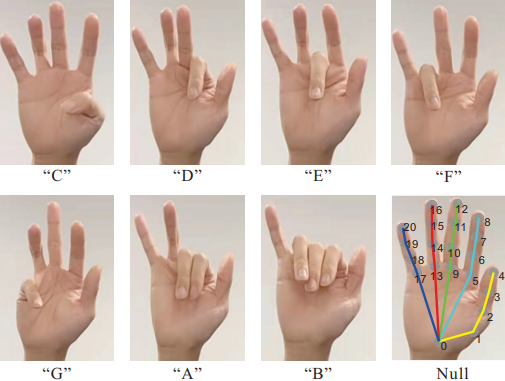
\includegraphics[width=\textwidth]{images/related-work/pitch-control}
	\end{subfigure}
	\hfill
	\begin{subfigure}{0.32\textwidth}
		\centering
		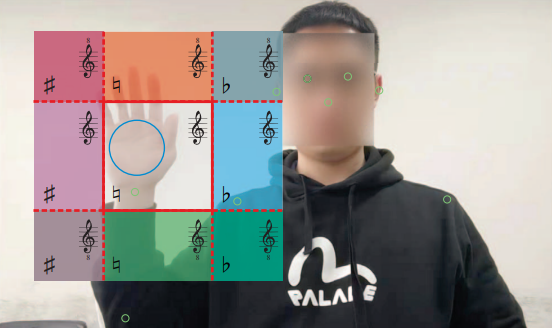
\includegraphics[width=\textwidth]{images/related-work/octave-control}
	\end{subfigure}
	\hfill
	\begin{subfigure}{0.32\textwidth}
		\centering
		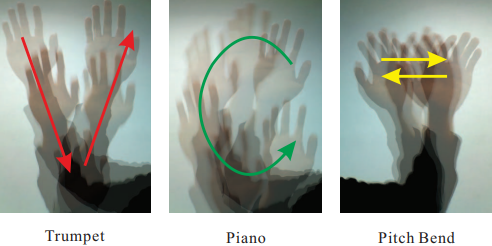
\includegraphics[width=\textwidth]{images/related-work/instrument-control}
	\end{subfigure}
	\caption{Instrument controls from~\protect\cite{hand-gesture-controlled-music-instrument}}
	\label{fig:instrument-control}
\end{figure}

In~\cite{emg-midi-controller}, an EMG based MIDI controller is implemented and tested.
The controller needs both a complex physical architecture and an intricate software to run.
The purpose of the controller is to identify four hand gestures, each associated with a different note.

The hardware consists of four components:
three EMG (Olimex Shield-EKG-EMG) sensors to be connected to the arm that is to act as the controller,
an Arduino UNO board to read the data from the three EMG sensors,
a Raspberry PI 4B board to receive the data from the Arduino and interpret it with the gesture recognition software,
and a computer that receives the final signal containing the MIDI note to be played.

The software communication between these devices is architected in the following way,
and is schematised in~\autoref{fig:emg-controller}.
First, the Arduino UNO board reads data from the three EMG sensors.
Then the Raspberry PI board requests this data from the Arduino, and when it receives it,
it passes it to the classifier that produces the hand gesture.
The result of the classifier is sento to the Arduino,
which converts it into a MIDI note and sends it to the computer so that the note can be played.

Three types of classifiers are used to test the system: Random Forest,
Support Vector Machines and a Neural Network with three hidden layers.
All three classifiers are trained on a dataset consisting of 60 measurements per each of the four gestures.

The results are unfortunately lower than hoped for,
with a maximum of 78\% obtained by SVM and a minimum of 71\% obtained by the Neural Network.
According to the authors, the cause for such a low result could be the Arduino,
which is deemed compromising for applications that require high sampling rates.

\begin{figure}[ht]
	\centering
	\begin{subfigure}{0.32\textwidth}
		\centering
		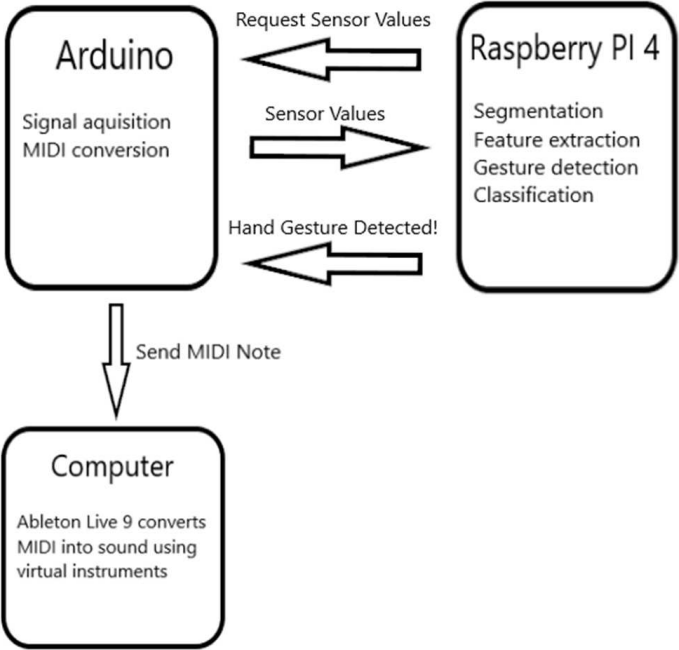
\includegraphics[width=\textwidth]{images/related-work/emg-architecture}
	\end{subfigure}
	\hfill
	\begin{subfigure}{0.32\textwidth}
		\centering
		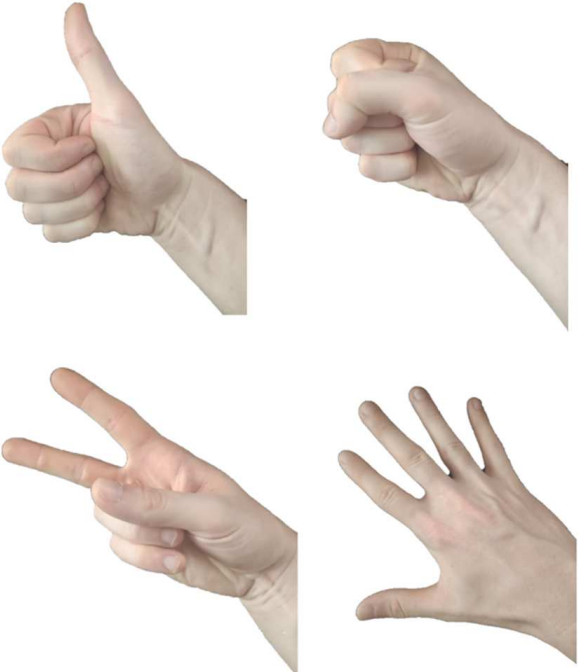
\includegraphics[width=\textwidth]{images/related-work/emg-gestures}
	\end{subfigure}
	\hfill
	\begin{subfigure}{0.32\textwidth}
		\centering
		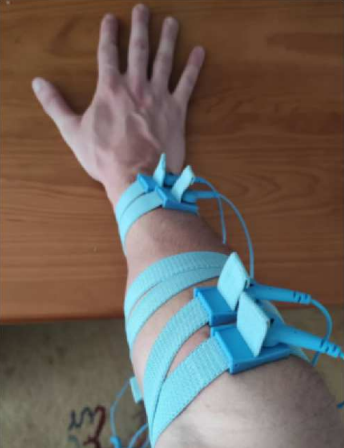
\includegraphics[width=\textwidth]{images/related-work/emg-sensors}
	\end{subfigure}
	\caption{Architecture, gestures and sensor position from~\protect\cite{emg-midi-controller}}
	\label{fig:emg-controller}
\end{figure}

\subsection{Virtual trainers}\label{subsec:virtual-trainers}
When it comes to learning a musical instrument using virtual reality tools,
it is not only important to have a tool that allows one to play
but also a tutoring system that gives feedback on the quality of the novice musician's performance.

The work done in~\cite{piano-fingering-recognition} is not exactly a virtual reality application, but still
represents an example of how depth sensors can be used for teaching and learning how to play a musical instrument.
This paper proposes a method for recognising piano fingering by analysing motion of multiple fingers through the use
of depth images acquired with a depth sensor.
The depth sensor used in the paper is a Microsoft Kinect, but in theory any other depth sensor may be used.

The proposed method consists of two modules: a learning module and a recognition module.
The learning module is used to generate a dataset of depth images for various key pressing patterns.
The recognition modules takes a depth image as input and tries the best matching key pressing pattern in the dataset,
with the goal to identify which one is being performed in the input depth image.
The recognition process uses the Nearest-Neighbor search technique.
Both the learning module and the recognition module make use of a background subtraction technique,
to separate the depth information about the keyboard from those about the hand.

The method was tested on three songs, with a dataset of 780 data elements in 130 classes acquired
by the learning module, obtaining a maximum recognition rate of 100\%, and a minimum of 91.6\%.
The recognition time was also measured and found to be 120 milliseconds per image,
making this method applicable to slow-tempo songs for piano beginners.

\begin{figure}[ht]
	\centering
	\begin{subfigure}{0.55\textwidth}
		\centering
		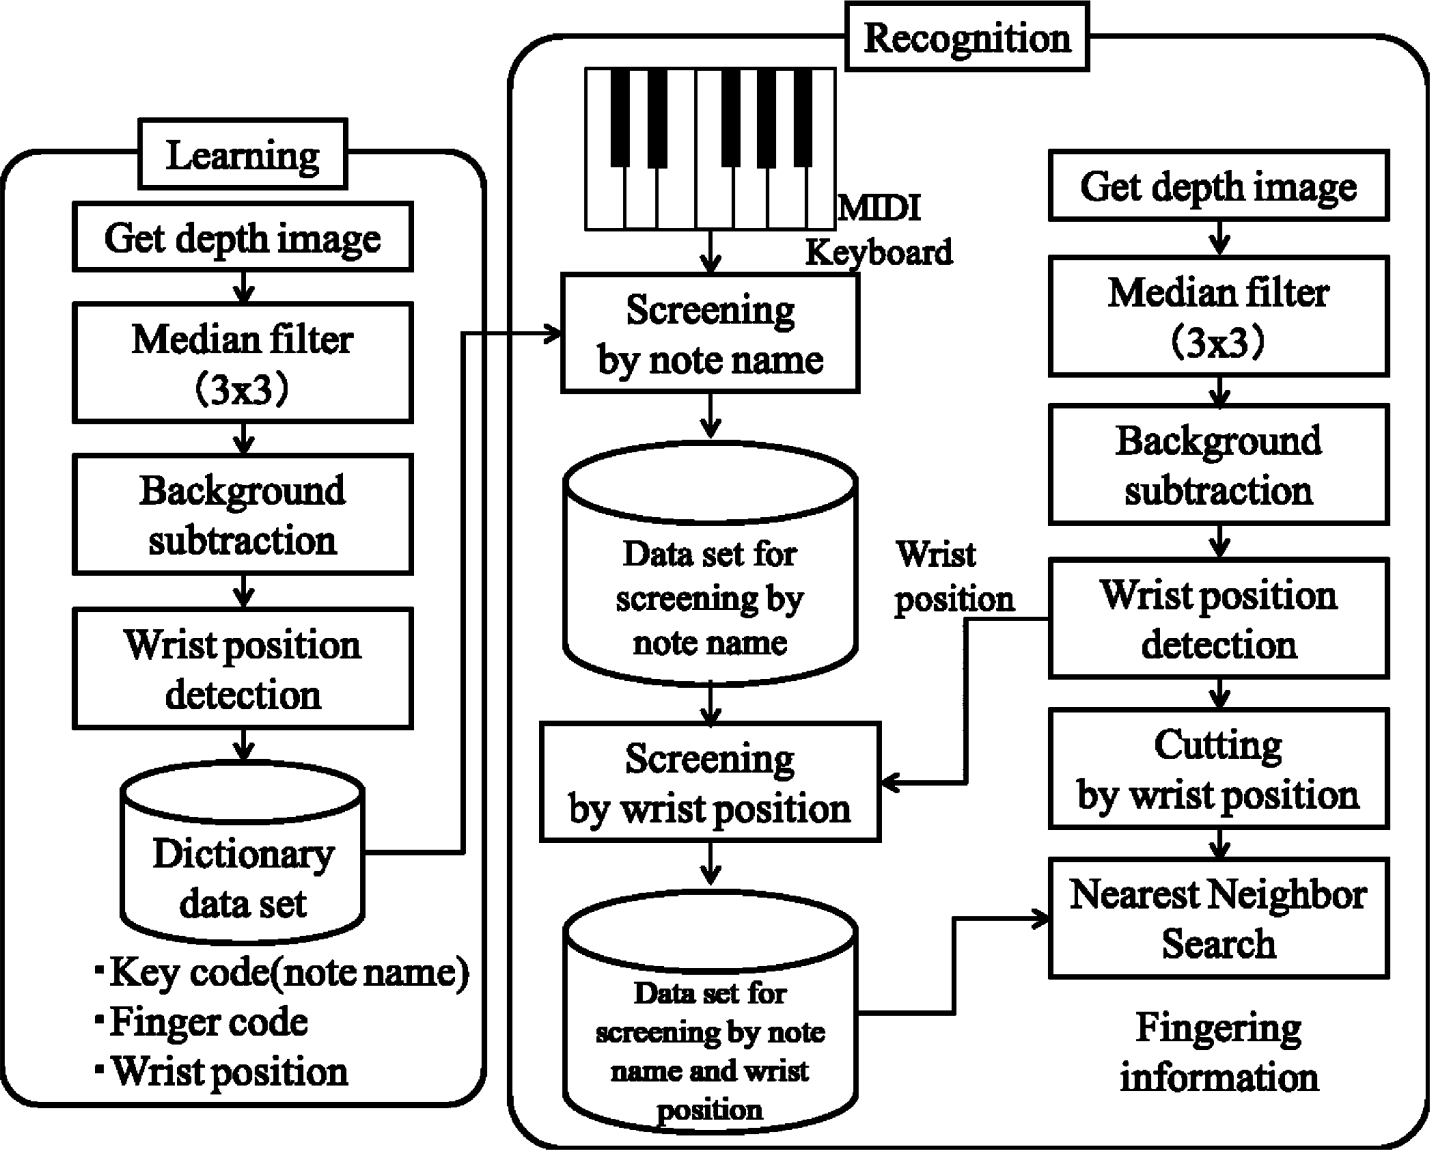
\includegraphics[width=\textwidth]{images/related-work/fingering-recognition-scheme}
	\end{subfigure}
	\hfill
	\begin{subfigure}{0.43\textwidth}
		\centering
		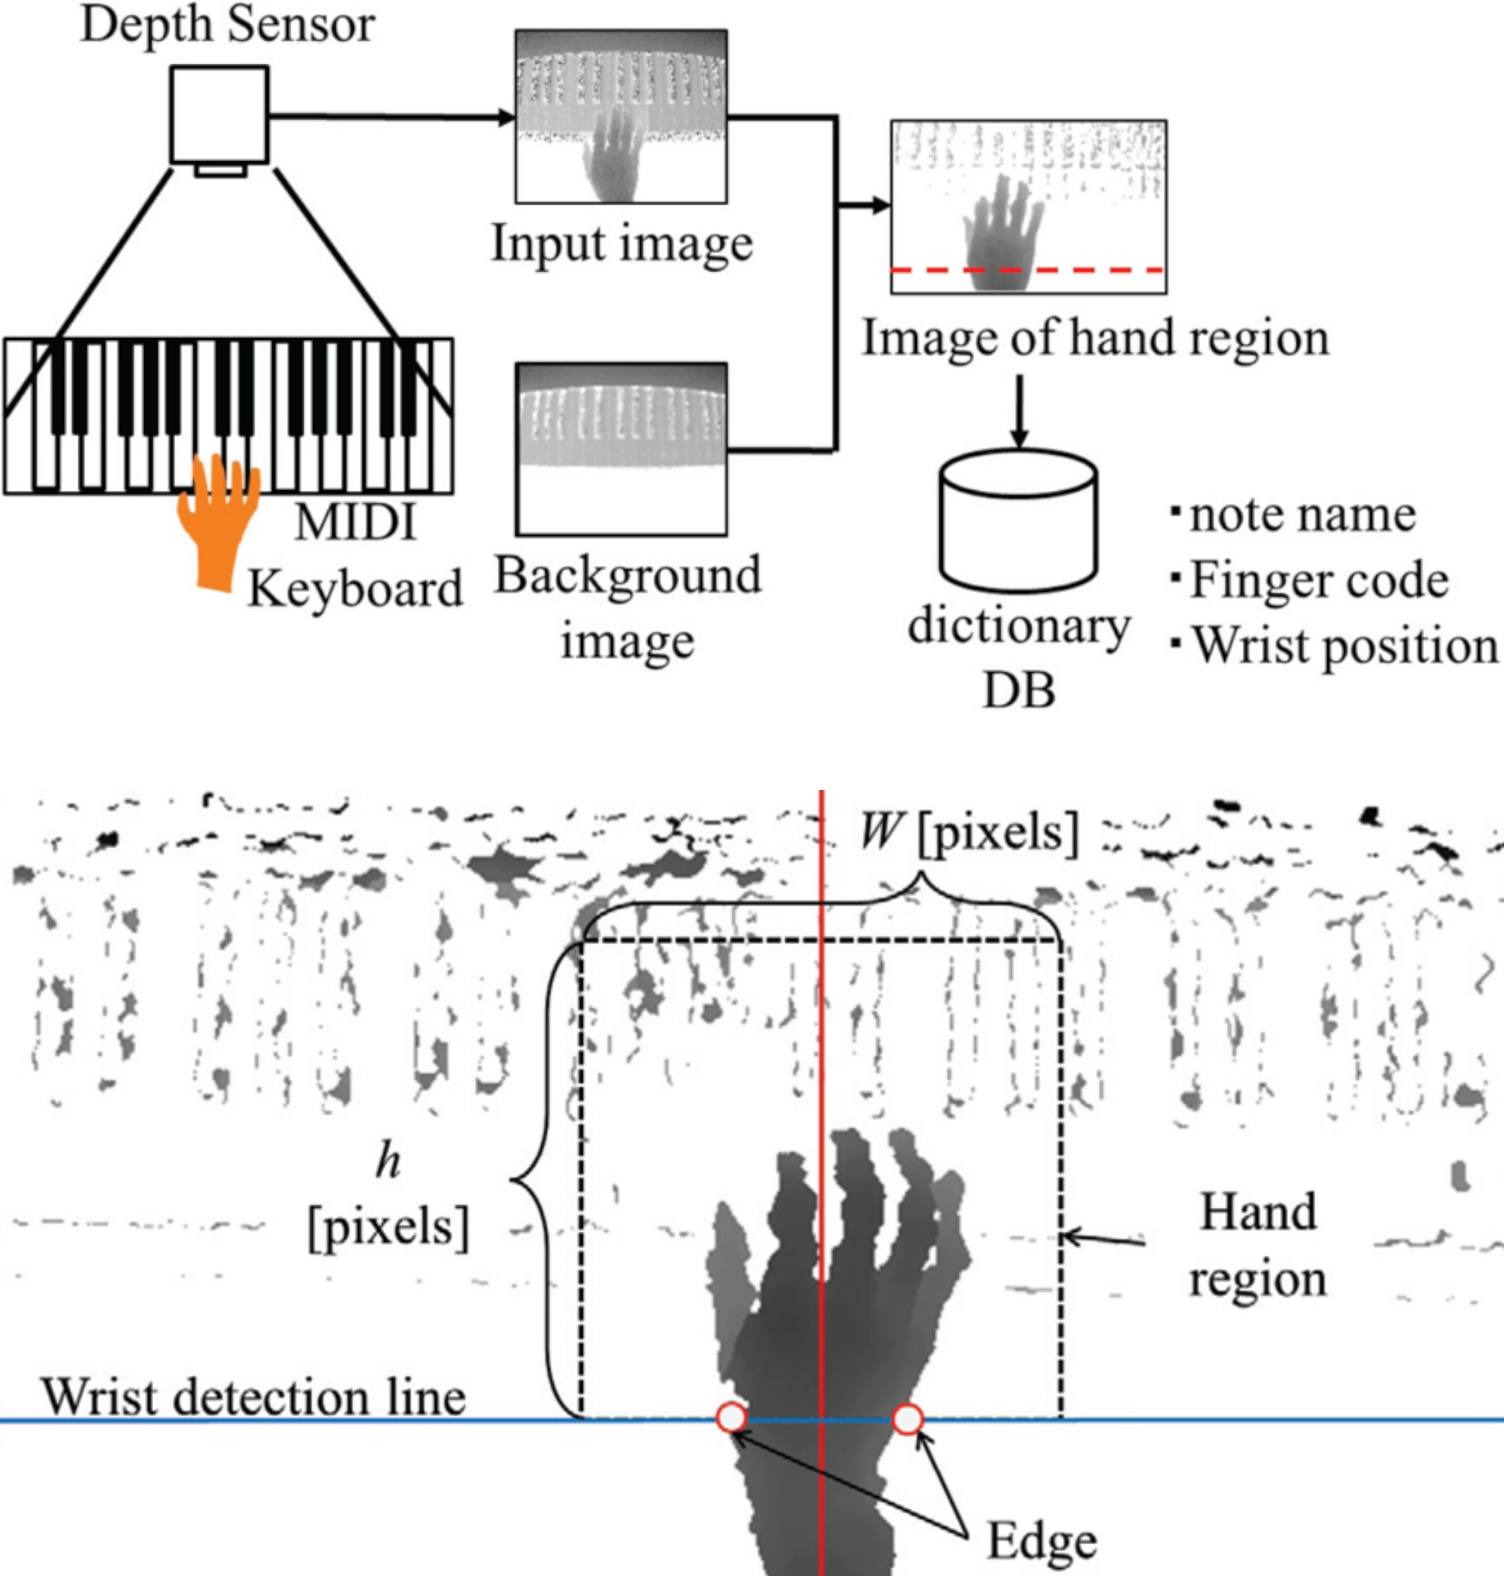
\includegraphics[width=\textwidth]{images/related-work/fingering-recognition}
	\end{subfigure}
	\caption{Architecture scheme, learning flow and recognition phase from~\protect\cite{piano-fingering-recognition}}
	\label{fig:fingering-recognition}
\end{figure}

In~\cite{fingering-generation}, an AR-based individual tutorial system is proposed.
Its goal is to automatically generate hand action animations
and displaying animations with real pianos using head-mounted displays.
Starting from a piece of music given as input, the system generates a coherent and natural-looking
animation of hands playing the given sequence of notes on a virtual piano.

To go from a MIDI file to an animation of hands playing a piano, two steps are taken.
The first step is to convert the raw MIDI file o a fingering-tagged MIDI file,
in which every note is tagged with the finger that plays it.
This is done with a Hidden Markov Model (HMM) and the Viterbi algorithm.
The HMM can be applied not only to single notes but also to chords that require a multi-finger movement.
The second step consists in creating the actual hand animation from the finger-tagged MIDI file.
The three patterns of fingering that can be recognised are Basic Finger Motion,
Alternative Finger Motion and Multi-finger Hand Motion.
To produce human-like animations for all these patterns,
the authors have defined step-by-step animations for each and every case above.

\begin{figure}
	\center
	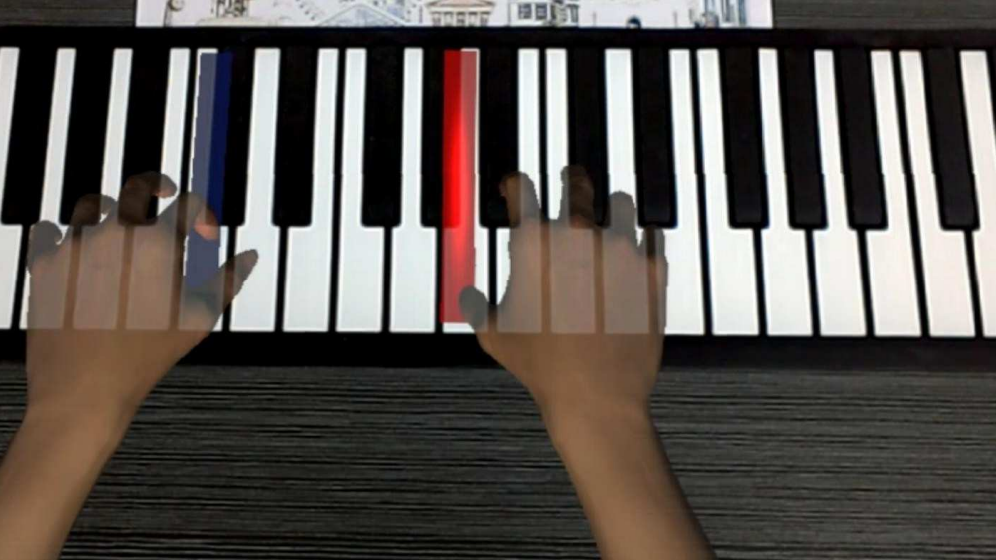
\includegraphics[width=0.7\textwidth]{images/related-work/fingering-generation}
	\caption{Fingering generation in an augmented reality environment from~\protect\cite{fingering-generation}}
	\label{fig:fingering-generation}
\end{figure}

Piano Beginner~\cite{piano-glove-training} is a finger training system with auditory and visual feedback (AVFB),
which supports both single-finger and multi-finger movements of two hands.
By wearing a pair of 5DT Data Glove Ultra and an optional VR headset, the user can experience an immersive simulation
of piano training.

The peculiarity of this project is in the setup phase:
rather than using a generic algorithm to detect finger pressure, the authors develop a calibration process
in which the user performs some actions like closing the hand and pressing each finger singularly,
to let the program learn what is the correct threshold to detect pressure for each finger.

The results of the experimentation show that users' accuracy increases by more than 20\% after 20 training sessions.

\begin{figure}[ht]
	\centering
	\begin{subfigure}{0.49\textwidth}
		\centering
		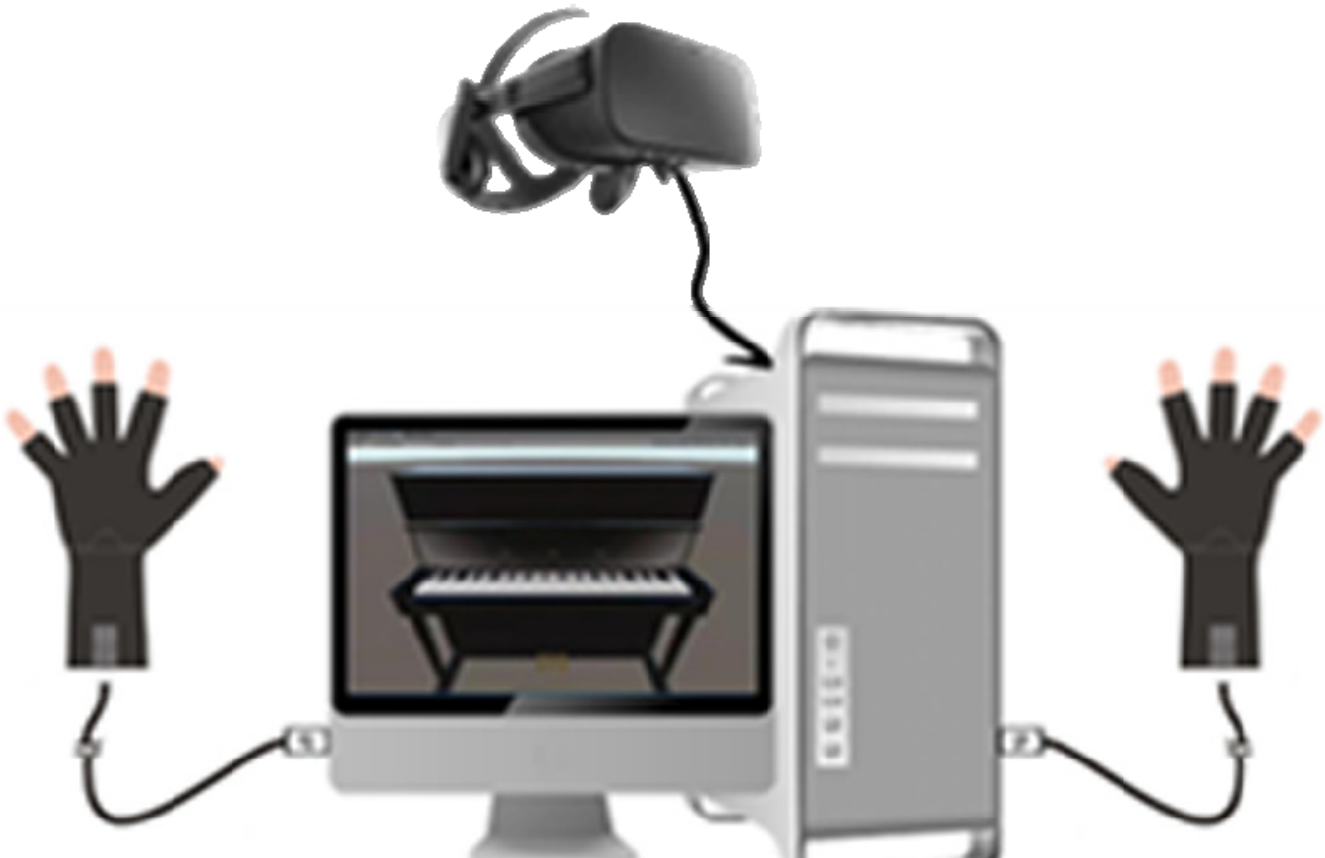
\includegraphics[width=\textwidth]{images/related-work/piano-glove}
	\end{subfigure}
	\hfill
	\begin{subfigure}{0.49\textwidth}
		\centering
		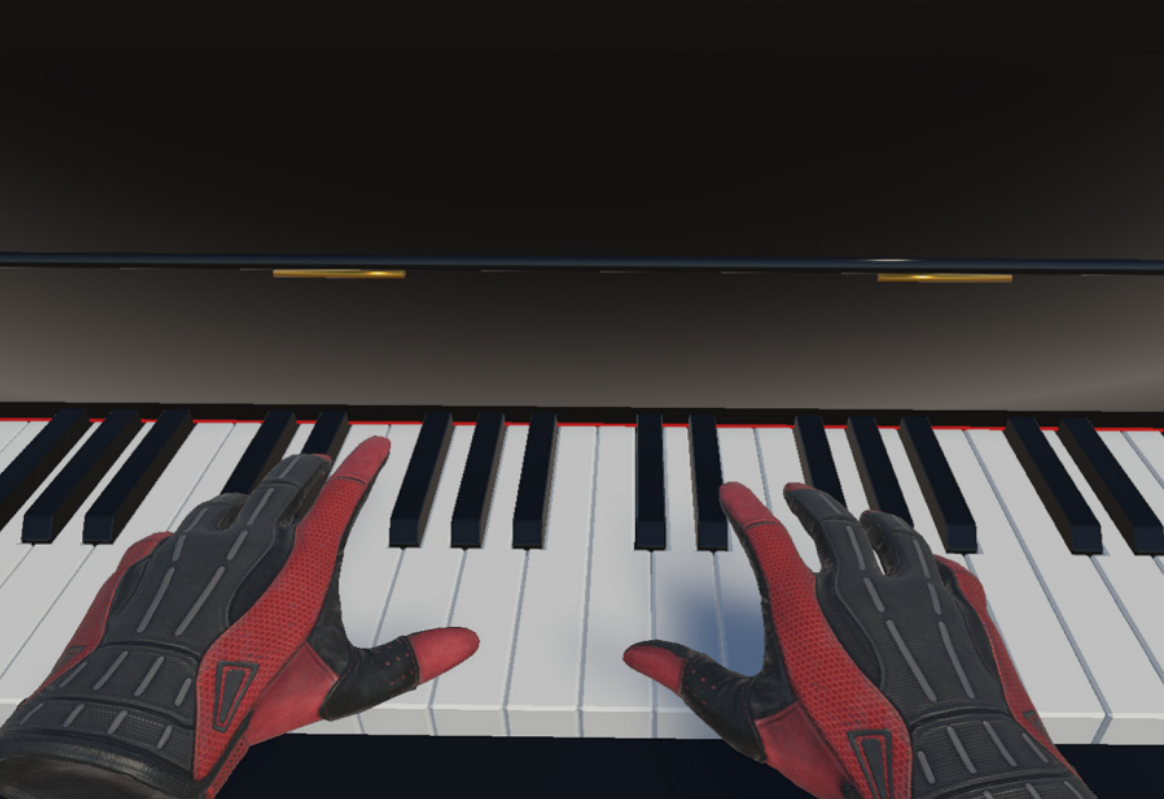
\includegraphics[width=\textwidth]{images/related-work/piano-glove-unity}
	\end{subfigure}
	\caption{Glove-based finger training system from~\protect\cite{piano-glove-training} and its Unity3D environment}
	\label{fig:piano-glove-training}
\end{figure}

GuitarGuru~\cite{guitar-guru} is a multi-featured application that caters for beginner guitarists with four
methods to learn and improve their performance on the guitar, combining computer vision and deep learning techniques.

The first feature allows a user to upload a video, or a link to a video on YouTube,
in which a musician plays the guitar.
GuitarGuru analyses the video and extracts all the chords from it in the form of a chord sheet.
With this function the user can also play the guitar in front of the webcam and get the chord sheets in real-time.

The second feature consists of a training session: the user selects a chord sheet from those previously
generated with the first feature, then starts the webcam and the application analyses their performance in real time,
evaluating its correctness and calculating the accuracy rate.

The third feature is similar to the previous but is a more specific and focused test on individual chords.
The user stands in front of the webcam and plays one chord at a time,
while the application measures the accuracy of each individual chord that is played.

The last feature is about music theory, offering a section where the beginner can learn notions about all the
music-related theories that will help the user in learning the basics of music,
including brief information about chords, scales, pitch, etc.

The dataset to train the deep learning model was built using python with OpenCV for preprocessing and MediaPipe for
extracting hand gestures, resulting in 25000 images: 5000 per each chord A, C, F, G, and 5000 representing a no-chord,
in which none of the previous chords was detected.
The deep learning model was built with Keras, with one input neuron and one output neuron,
32 filters in each layer and the size of a layer being (5, 5) with Relu as the activation function.

The model gives an accuracy of 97.09\% for the 4 chords A, C, F, G and a loss of 2.91\%.
In the future, more chords can be added for identification,
which would help expand the range of music genres to which GuitarGuru can be applied.

\begin{figure}[ht]
	\centering
	\begin{subfigure}{0.60\textwidth}
		\centering
		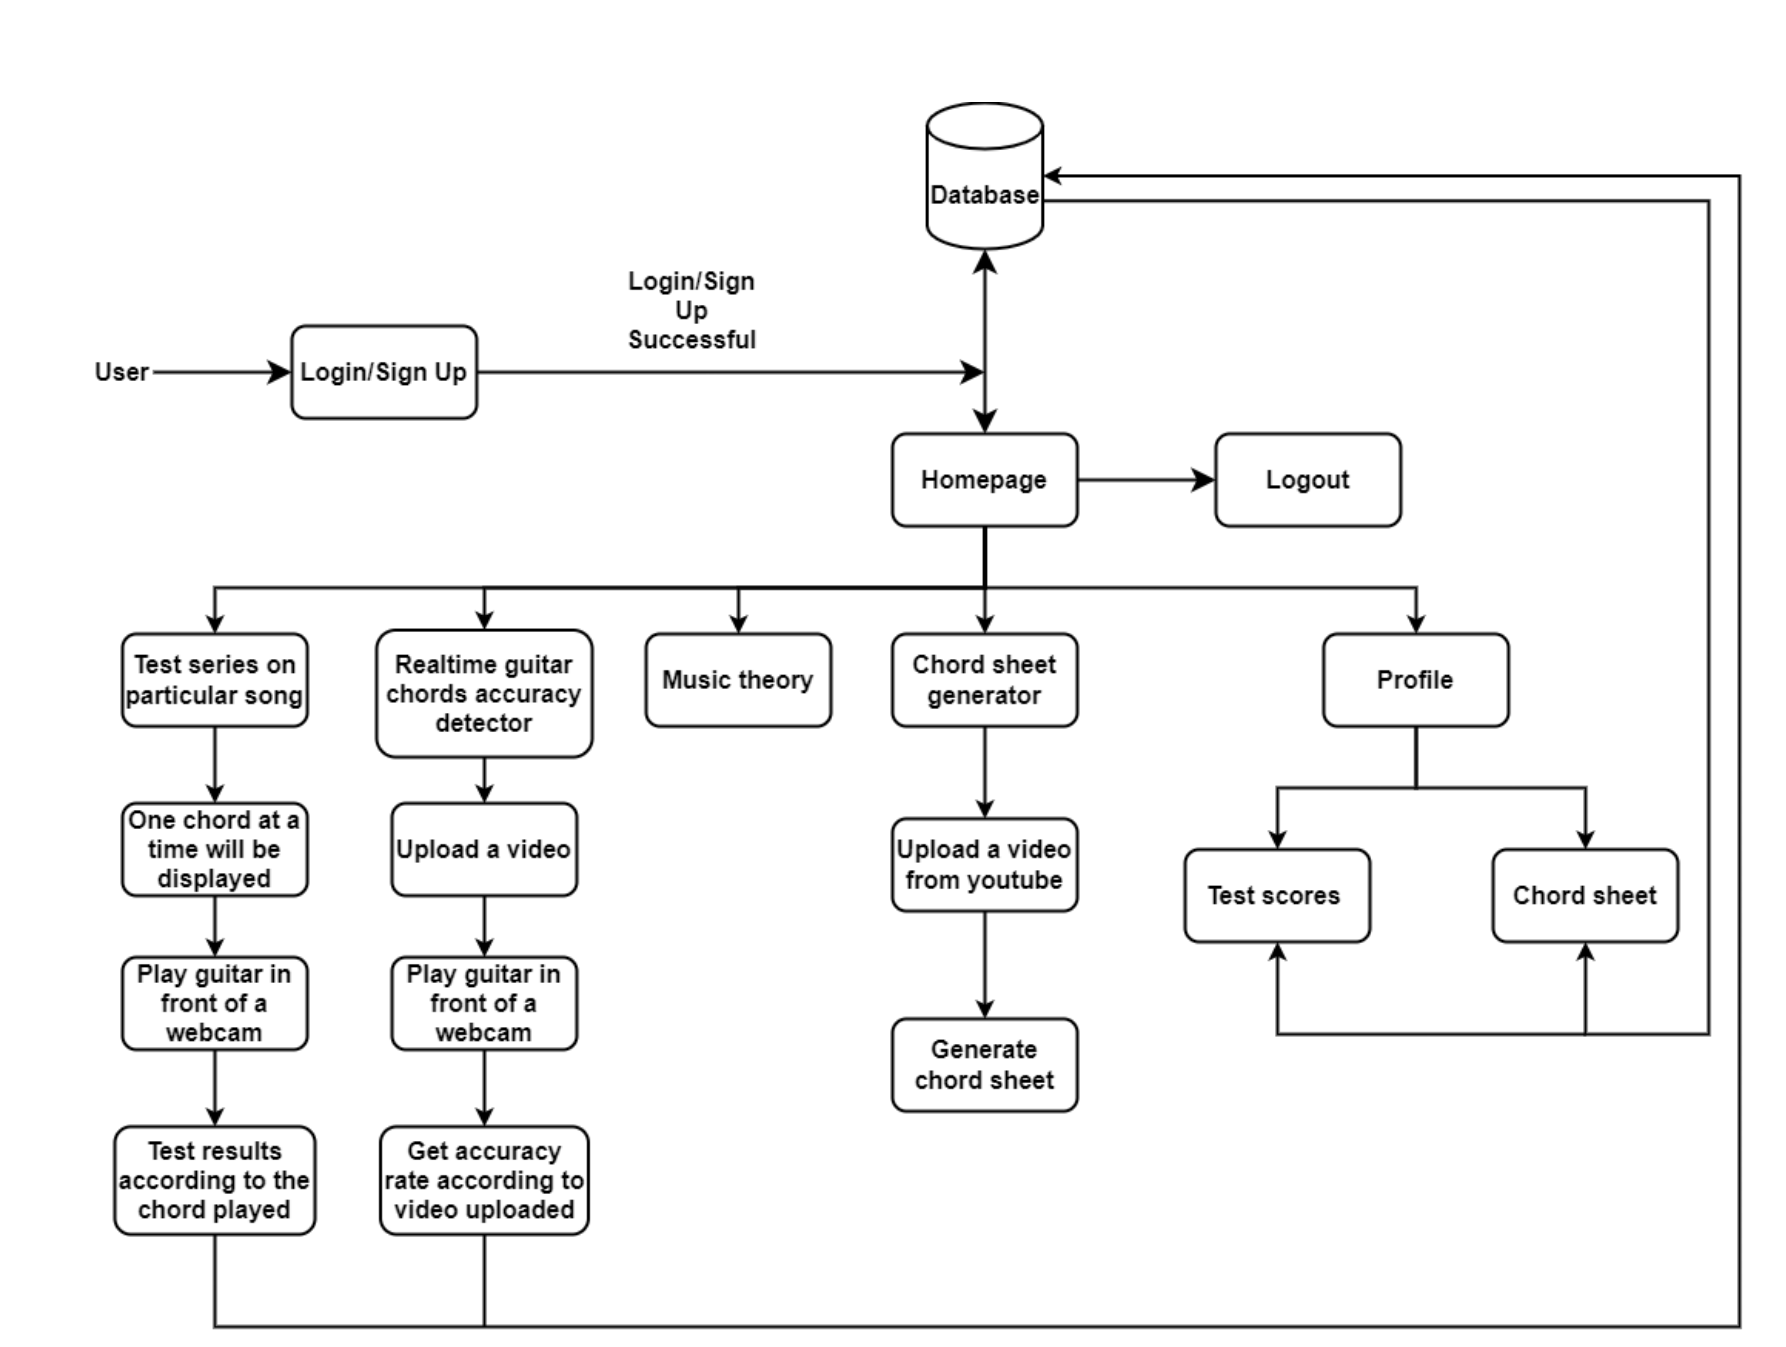
\includegraphics[width=\textwidth]{images/related-work/guitar-guru}
	\end{subfigure}
	\hfill
	\begin{subfigure}{0.39\textwidth}
		\centering
		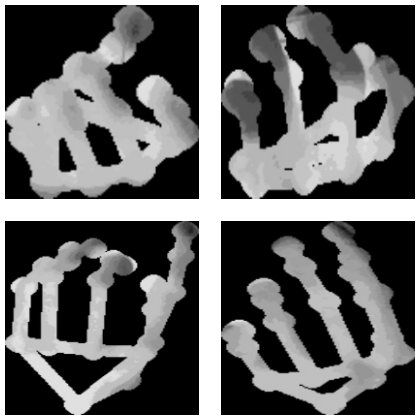
\includegraphics[width=\textwidth]{images/related-work/guitar-guru-chords}
	\end{subfigure}
	\caption{Architecture scheme and 4 chords (A, C, F, G) recognised from~\protect\cite{guitar-guru}}
	\label{fig:guitar-guru}
\end{figure}

Another trainer for pianists can be found in VRmonic~\cite{vrmonic-piano-trainer}, an immersive VR-based piano trainer
that uses the Unity Game Engine and a VR headset with a hand detector to compare the user's hand movements to the ones
of a virtual expert oracle, on a set of 48 scales for each of the 12 notes.
The goal of this project is not only to teach how to play the piano, but also how to play it with the
correct hand form, preventing long-term injuries in musicians of all levels.

The oracle's hand poses are recorded using a capture environment
in which some expert pianists perform the scales on an 88-key piano.
The pianist's hands are captured using a Microsoft Azure RGB-D camera mounted 88.25 cm above the piano.
Five trials are performed for each scale and the resulting joint positions are merged together into the final oracle positions by averaging the positions in each trial.

When running a training session, the user needs any VR headset that supports Unity and is capable of doing hand detection.
After having selected the note, scale, and beats per minute, the user can start to record a playback or run a playback by the oracle.
Pieces recorded by the user can be later played back together with the ones played by the expert oracle, creating an overlay of two pairs of hands, one belonging to the user and one to the oracle.
The user can set the tolerance level, which represents the number of collisions between corresponding joints on the two pairs of hands, to control the level of feedback on alignment with the expert.
VRmonic currently does not support real-time feedback.

VRmonic is a promising project with great potential.
Future development possibilities include adding support for real-time feedback mode,
the incorporation of qualitative feedback via large language models (LLM) to provide personalised voice-based
feedback based on the magnitude of the error, and the addition of further control over the pianist's posture
as well as the position of his hands.

\begin{figure}[ht]
	\centering
	\begin{subfigure}{0.55\textwidth}
		\centering
		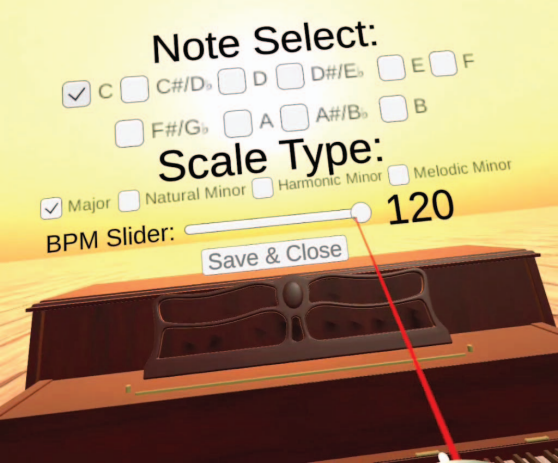
\includegraphics[width=\textwidth]{images/related-work/vrmonic}
	\end{subfigure}
	\hfill
	\begin{subfigure}{0.43\textwidth}
		\centering
		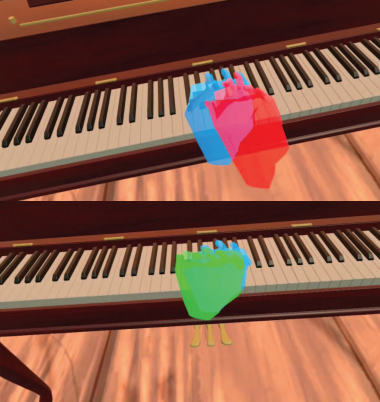
\includegraphics[width=\textwidth]{images/related-work/vrmonic-example}
	\end{subfigure}
	\caption{VRmonic interface and overlapping hands example: inaccurate vs accurate}
	\label{fig:vrmonic}
\end{figure}
